\chapter{Experiments}

The following sections discuss a series of experiments relating to the discussed methods. 
We first introduce a series of simulation experiments to verify and compare the results with a known distribution.
We then discuss some experiments relating to improving the SGHMC through better estimation of the variance $\hat{V}$.
Finally, we apply the methods discussed to some deep learning problems using the MNIST and CIFAR10 datasets.

\section{Simulated data}

To verify the implementation of the MCMC methods, we carry out some simulation experiments.
The first experiment is a recreation of an experiment from the original SGHMC paper, where they sample from a bimodal distribution with $\log p(x) \propto 2 x^2 - x^ 4$ with different configurations. 
First, the distribution is sampled from as-is, using regular HMC.
Then the batched dynamics in \cref{eq:sghmc-model} are simulated by adding simulated noise $\epsilon \sim \mathcal{N}(0, 4)$ to the gradient during the sampling process. 
We thus fulfill the distributional assumptions of SGHMC exactly and may also use the known noise scale as the noise estimate for SGHMC. 
With this introduced noise we also investigate the naive approach to using HMC, both with and without using an MH step. 
The resulting sampled distributions can be seen in \cref{fig:synthetic}
\begin{figure}[htb]
    \centering
    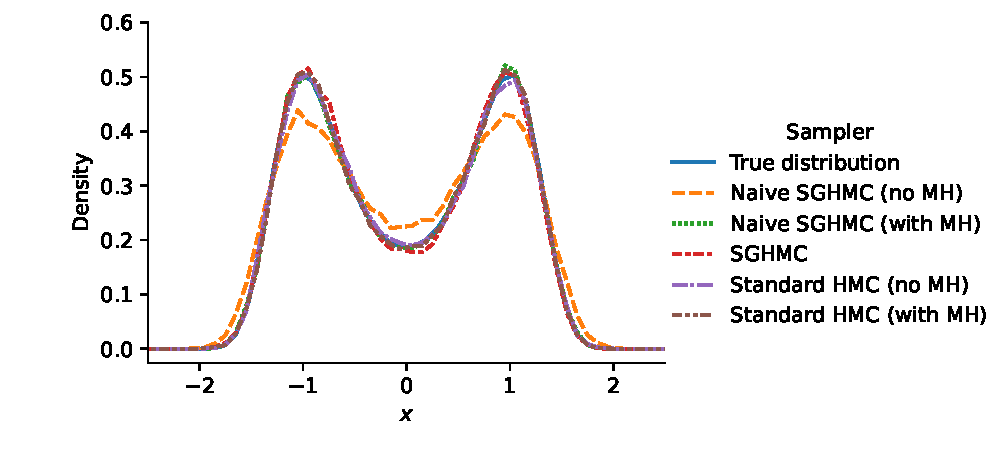
\includegraphics[width=0.9\textwidth]{Figures/synthetic.pdf}
    \caption{Samples from $\log p(x) \propto 2 x^2 - x^ 4$ for different sampling configurations}
    \label{fig:synthetic}
\end{figure}
These results are similar to those of the SGHMC paper and seem to verify that our implementation is correct.
We also see that the sample distributions from both the standard HMC sampler and the SGHMC sampler closely resemble the accurate distribution. 
The naive SGHMC sampler does seem to break down when we do not include an  MH step, and since we also compare with the regular HMC with no MH step, this demonstrates that it may not be purely down to omitting the MH step. 

If we include an MH step, the naive approach also seems to work; however, we are not adding any noise to $E(\cdot)$ when performing the MH step, corresponding to calculating $E(\cdot)$ across the whole data set. 
This approach is impractical in the context of deep learning.
In the next experiment, we will implement a naive alternative approach, where each MH step is performed based on each batch of data. 
This experiment also does not address whether noise the dynamics of \cref{eq:sghmc-model} are even reasonable as a model for the noise introduced through batching the gradient. 

In order to address these points, we perform an additional simulation experiment. 
This is also to demonstrate the relevance of the different methods in the context of MCMC inference.
We consider the polynomial model of $P(x) = -x + \frac{1}{2}x^2 + \frac{1}{3}x^3$, 
and with $\epsilon \sim \mathcal{N}(0, 1)$, consider a set learning points $y_i = P(x_i) + \epsilon$ for $i=1,\dots,15$, where $x_i$ are linearly spaced over the interval $[-3, 3)$ with a small amount of noise added. 
We then consider the problem of bayesian polynomial regression with known noise $\sigma=1$ and the regression model:
\begin{align*}
    P(x) = a_0 + a_1 x+a_2 x^2 + a_3 x^3
\end{align*}
where each parameter are given a $\mathcal{N}(0, 1)$ prior.
The exact parameter posterior $p(a|x,y)$ for this regression problem is known, and can therefore be compared to the sampled distribution of the samplers. 
More specifically, three sampling strategies are considered, regular HMC conditioned on all data points, HMC where each sample is based on a batch of 5 observations, and SGHMC also with batches of 5 observations.
For demonstration, plots the joint distribution of $a_1$ and $a_3$ as sampled by the different setups can be seen in \cref{fig:simulated_joint_comp}.
\begin{figure}[htbp]
    \centering
    \begin{subfigure}[b]{0.45\linewidth}
        \centering
        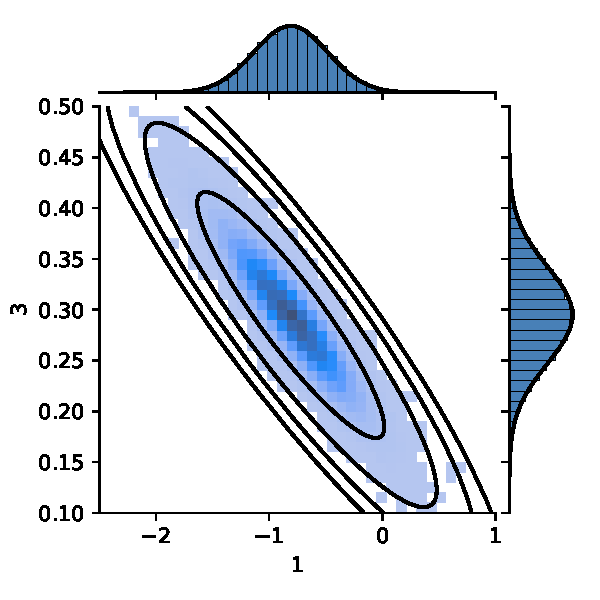
\includegraphics[width=\linewidth]{Figures/simulated_joint_HMC_15.pdf} 
        \caption{HMC conditioned on all data points.}
    \end{subfigure}
    \begin{subfigure}[b]{0.45\linewidth}
        \centering
        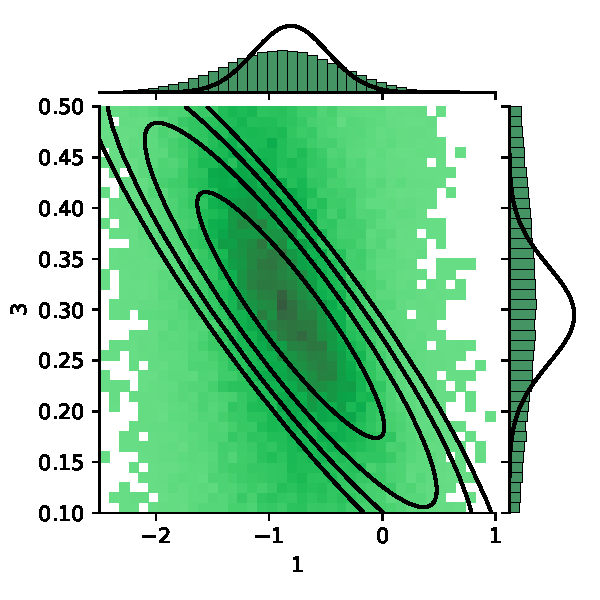
\includegraphics[width=\linewidth]{Figures/simulated_joint_HMC_5.pdf} 
        \caption{HMC with batch size 5}
    \end{subfigure}
    \begin{subfigure}[b]{0.45\linewidth}
        \centering
        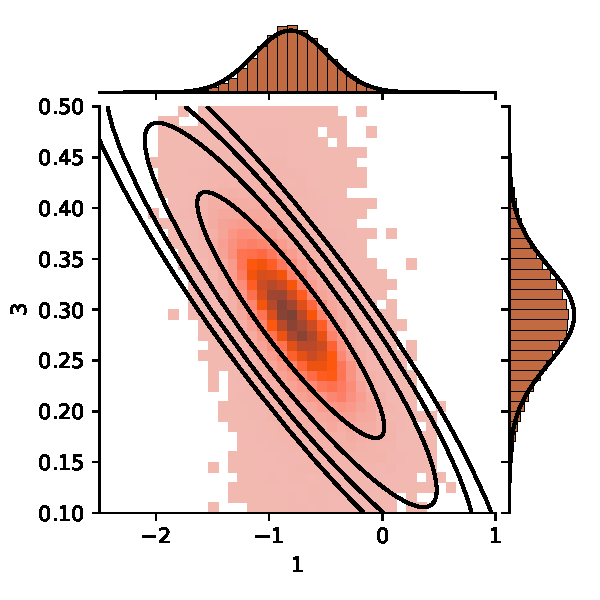
\includegraphics[width=\linewidth]{Figures/simulated_joint_SGHMC_5.pdf} 
        \caption{SGHMC with batch size 5}
    \end{subfigure}
    \caption{Joint distribution of samples for $a_1$ and $a_3$ for the polynomial regression example for HMC and SGHMC for different batch sizes, with the actual posterior density also shown.}
    \label{fig:simulated_joint_comp}
\end{figure}
Figures showing the sampled joint distribution for every pair of parameters, for each algorithm can be found in \cref{apx:simulated-joint}.
We find that the also this naive approach SGHMC does not correcly sample from the posterior dsitribution.
The actual SGHMC algorithm also does not seem to sample exactly from the posterior, with some overdispersion present in samples compared to the unbatched HMC. 
This overdispersion is however minimal compared to the naive implementation.
Later, we will discuss a possible improvement upon this algorithm, based on actually proving an estimate of the gradient variance.

\subsection{Variational Inference} 
We can also repeat the experiment above using the variational inference framework.
A comparison of the pairwise marginal distributions for the true posterior and the variational posterior is shown in \cref{fig:vi-simulated}. 

Since we assume independent variables for the variational posterior, the fit is not particularly good compared to the MCMC methods. 
However, this still serves to verify that the implementation is behaving as expected.
\begin{figure}[htbp]
    \centering
    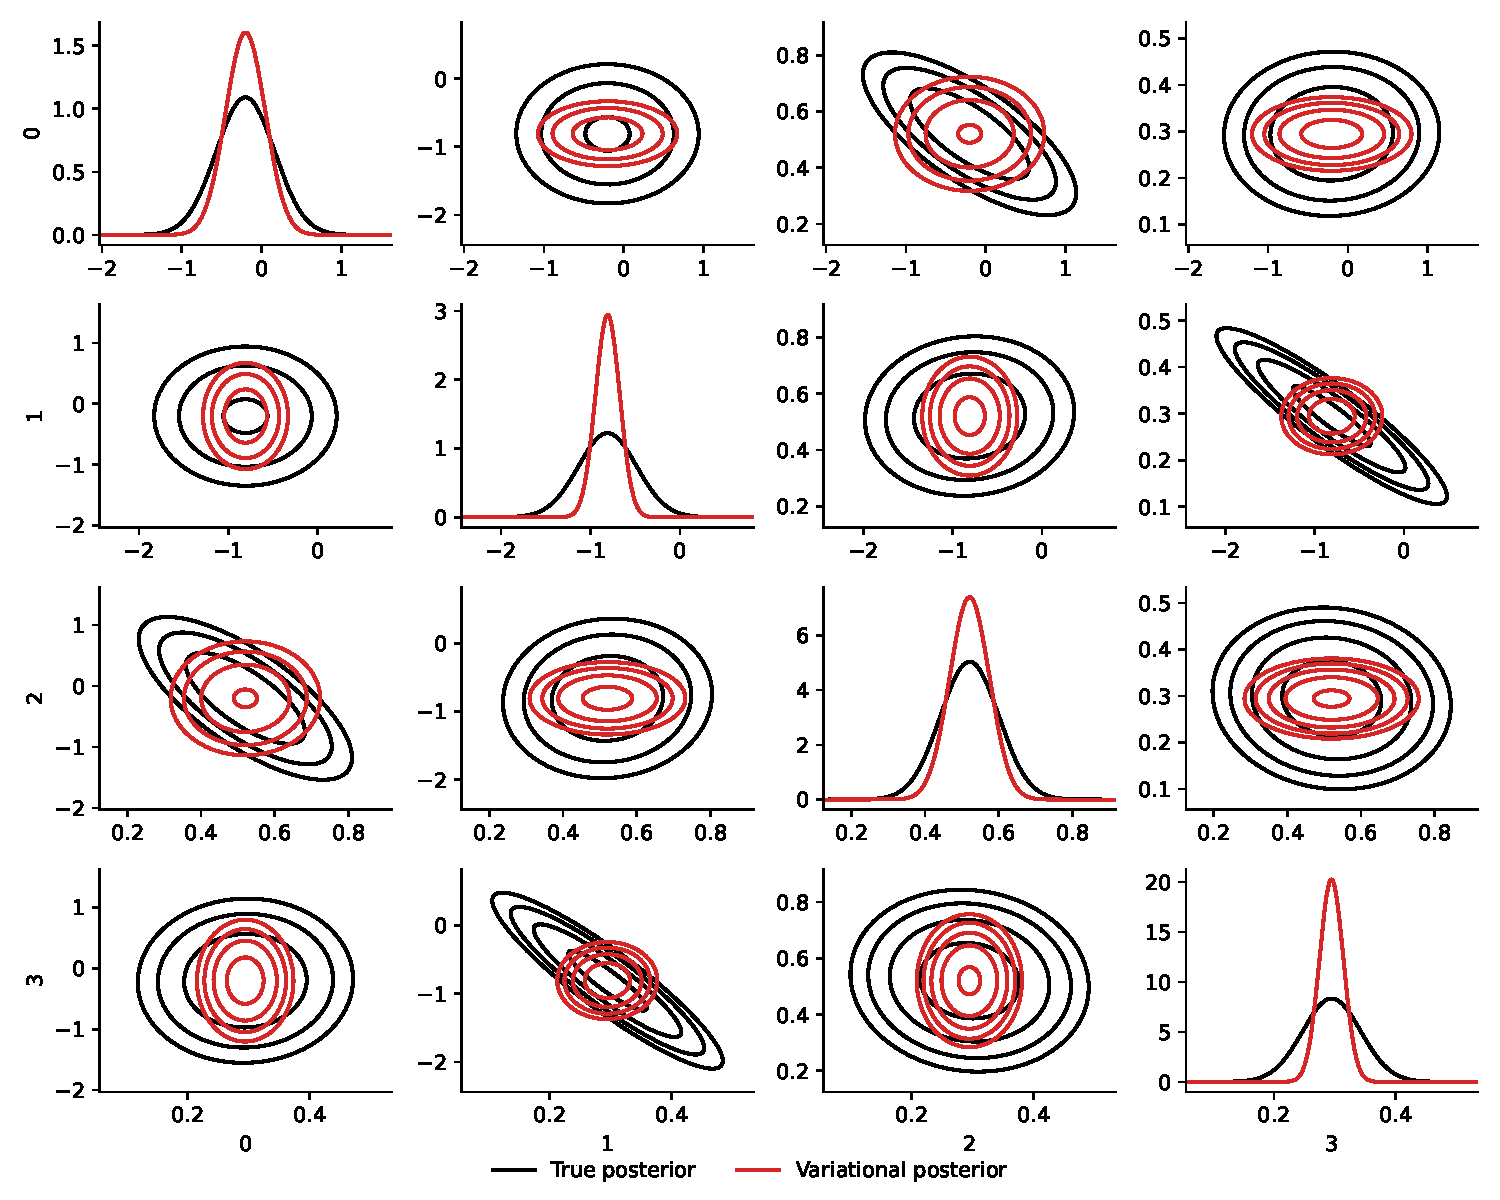
\includegraphics[width=\linewidth]{Figures/vi-simulated.pdf}
    \caption{Variational posterior compared to true posterior for Bayesian polynomial regression example.}
    \label{fig:vi-simulated}
\end{figure}


\section{Estimating the variance}

In the SGHMC paper, they propose estimating the variance introduced through batching as $\hat{V}=0$ and then relying on the known simulated noise to make the inaccuracy of this estimate irrelevant. 
However, it seems worth investigating whether we could improve performance by providing an actual estimate of the variance instead. 
The SGHMC paper also mentions this idea; however, they do not explore it further. 

Since we use an upper bound $C$ on the noise variance, parameterized by $\alpha$, we may end up with estimated noise larger than the upper bound.
Adjusting the upper bound $C$ to accommodate this would also require adjusting the $\alpha$ parameter accordingly.
Since the $\alpha$ corresponds to the momentum decay of the algorithm, we may end up with unstable behavior, especially for $\alpha > 1$. 
Instead, we fix the parameter $\alpha=\epsilon M^{-1}C$ and adjust the mass matrix $M$, implicitly adjusting $C$ as well.
With $M = M_0 W$ were $W$ is a diagonal matrix of weights, we can then, depending on the variance estimate, rescale the mass such that the upper bound $\alpha$ is sufficiently above the estimate $\hat\beta$, e.g., by some factor $m_{\text{est}}$.
If we let the learning rate be given as $\eta_0$  for the unscaled mass matrix with $W = I$, then the learning rate for the scaled system can be found as $\eta = \epsilon^2 M^{-1} = \epsilon^2 M_0^{-1}W^{-1} = \eta_0 W^{-1}$, and
\begin{align}
    m_{\text{est}} \cdot \hat{\beta}  &\leq \alpha \Leftrightarrow\\ 
    m_{\text{est}} \cdot \frac{1}{2} \hat V \eta   &\leq \alpha \Leftrightarrow\\ 
    m_{\text{est}} \cdot \frac{1}{2} \hat V \eta_0 W^{-1}  &\leq \alpha \Leftrightarrow\\ 
    m_{\text{est}} \cdot \frac{1}{2\alpha} \hat V \eta_0   &\leq W.
\end{align}
We can ensure that the above inequality is satisfied by setting the entries in $W$ as follows:  
    \begin{align}
    W_{i,i} &= \begin{cases}
        1 & \frac{1}{2\alpha}m_{\text{est}} \eta_0 \hat{V}_{i,i} < 1, \\
        \frac{1}{2\alpha}m_{\text{est}} \eta_0 \hat{V}_{i,i}, & \text{otherwise}.
    \end{cases}
\end{align}
The sampler then rescales the system mass matrix based on the variance estimates every once in a while, e.g., every 50 samples.
When updating from $W$ to $W^\prime$, we also rescale the $\nu=\epsilon M^{-1}r$ parameter accordingly with $W/W^\prime$.
If the variance estimates $\hat \beta$ happen to be greater than $\alpha$ in between the mass rescaling, we clamp the estimate at the upper bound $\alpha$ and add no additional noise. 

This method of rescaling the mass matrix is in a sense similar to the approach outlined in \cite{wenzel_how_2020}, where they also include a step calculating a preconditioning matrix, ie.
They found that using the preconditioning step generally improved sampling performance.


There are multiple ways to go about obtaining the actual variance estimate.
We could try to calculate a running variance statistic using the within batch sample variance of the gradients:
\begin{equation}
    \frac{1}{|\tilde{\D}|-1}\sum_{(x_i,y_i)=\tilde{\D}} (\nabla U(\theta; x_i, y_i) - \nabla \bar{U}(\theta))^2
\end{equation}
and then scale the variance up to the fit the batch size. 
The main issue we found with this approach is that calculating the gradient for each observation individually within a batch is not that efficient.
While it may be possible to calculate the statistic above using a backpropagation framework such as autograd without doing a backward pass for each observation, it is not trivial since autograd only allows for calculating gradients of scalars. 

Instead, we look at three other approaches. 
The first approach is to run through some number of training batches before each epoch, calculating the gradient for each batch keeping the parameters constant. 
A variance estimate is then calculated based on these gradients and used for the following epoch.

The two other approaches instead keep track of running statistics. 
The first is inspired by  ADAM algorithm \cite{kingma_adam_2017} and uses exponentially decaying running estimates of the mean, $m_t$ and variance, $v_t$.  
Since the ADAM algorithm does not center the second-moment estimate, we subtract the squared mean, such that the variance estimate becomes as $v_t - m_t^2$, clamping the estimates from below at zero.

Finally, we also try a variation on the running statistics of the ADAM ,algorithm.
This approach uses the first moment to center the second-moment estimates, updating the estimates $v_t,m_t$ using the observed gradient $g$  for some $\alpha\in(0,1)$ as follows:
\begin{align}
    d &\gets g - m_t \\
    i &\gets \alpha \cdot d \\
    m_{t+1} &\gets m_t + d \\
    v_{t+1} &\gets (1 - \alpha)\cdot  (v_t +  d\cdot i).
\end{align}
This approach is described in \cite{finch_incremental_nodate}.

In order to test these three different approaches, we apply them to the simulated example from the previous section.
For every ten samples, the gradient variance is estimated using 100 random batches from the training data set.
This estimate is then compared to the estimates provided by the different estimators. 
compared to the observed variance can be seen in \cref{fig:est_variances_simulated}.
\begin{figure}[htbp]
    \centering
    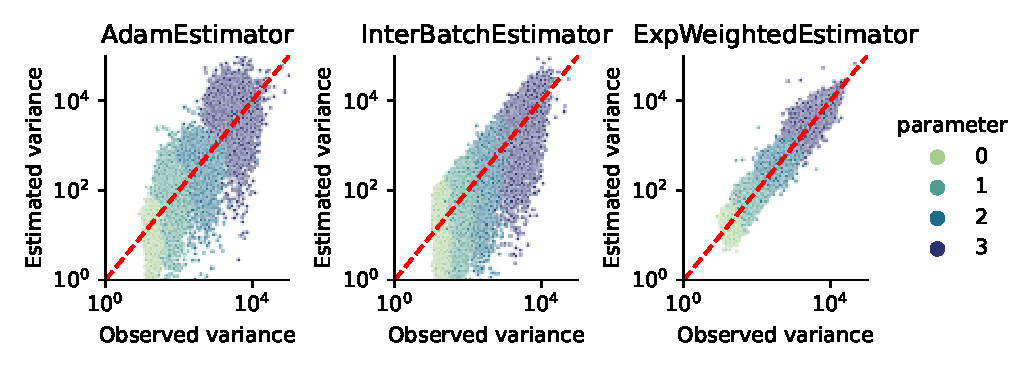
\includegraphics[width=\linewidth]{Figures/simulated_sghmc_gradient_variance_estimations.pdf}
    \caption{Estimated variance compared to observed variances across 100 batches.}
    \label{fig:est_variances_simulated}
\end{figure}
\begin{table}[htbp]
    \centering
    \begin{tabular}{lrrrr}
\toprule
parameter &    0 &    1 &    2 &    3 \\
variance\_estimator   &      &      &      &      \\
\midrule
AdamEstimator        & 0.65 & 2.03 & 1.67 & 2.98 \\
ConstantEstimator    & 1.00 & 1.00 & 1.00 & 1.00 \\
ExpWeightedEstimator & 0.30 & 0.41 & 0.42 & 0.49 \\
InterBatchEstimator  & 1.00 & 0.98 & 0.98 & 0.94 \\
\bottomrule
\end{tabular}

    \caption{Relative errors for estimation of gradient variance compared to observed variance across 100 batches, for the different estimation schemes,}
\end{table}
Note that we plot these values using a logarithmic scale, so the estimates may seem better than they are, especially concerning overestimations. 
It may still be that they are better than simply setting $\hat\beta=0$ in terms of estimating the posterior correctly.
In \cref{fig:simualted_var_est_joint_comp}, the sampled marginal distribution of $a_1$ and $a_3$ are shown again, now compared SGHMC with and without a variance estimator.
\begin{figure}[htbp]
    \centering
    \begin{subfigure}[t]{0.45\linewidth}
        \centering
        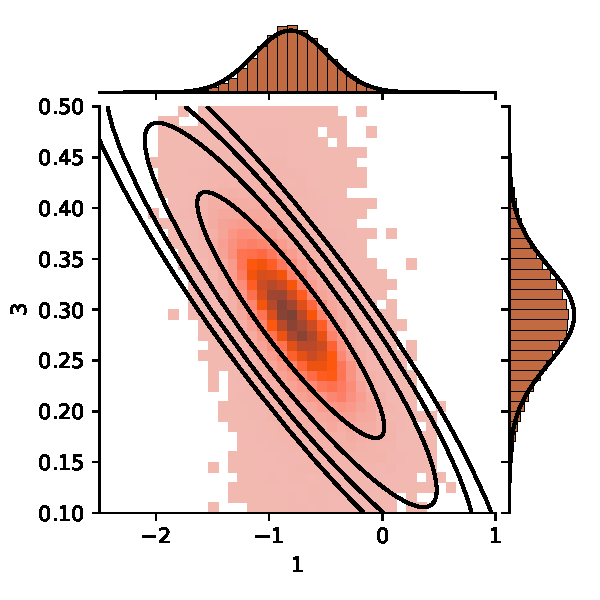
\includegraphics[width=\linewidth]{Figures/simulated_joint_SGHMC_5.pdf} 
        \caption{SGHMC with with gradient variance estimated as $\hat{V}=0$.}
    \end{subfigure}
    \begin{subfigure}[t]{0.45\linewidth}
        \centering
        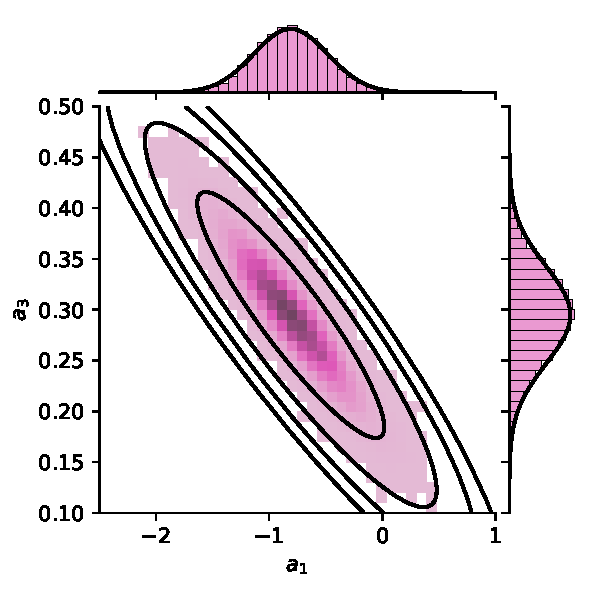
\includegraphics[width=\linewidth]{Figures/simulated_var_est_joint_ExpWeightedEstimator.pdf} 
        \caption{SGHMC with using the exponentially scaled estimator of gradient variance}
    \end{subfigure}
    \caption{Joint distribution of samples for $a_1$ and $a_3$ for the polynomial regression example for HMC and SGHMC for different batch sizes, with the actual posterior density also shown.}
    \label{fig:simualted_var_est_joint_comp}
\end{figure}
In this case, it does seem like estimating the variance can improve the accuracy of the sampler.
This improvement may come down to the fact that the sampler with gradient estimation can reduce the step size, lowering discretization and batch error compared to SGHMC without an estimate. 

\subsection{Marginal distribution of momentum}

In \cite{wenzel_how_2020}, they propose using the marginal distribution of the momentum as a test of the sampling assumptions. 
Per the dynamical system, if we simulate the system precisely, the marginal distribution of $r$ should be $\mathcal{N}(0, M^{-1})$. 
We should therefore see $r M^{-1/2} \sim \mathcal{N}(0, I)$. 
Applying the inner product, we arrive at so-called \emph{kinetic temperature} $T_K(r) = \frac{r^T M r}{d}$.
The kinetic temperature then follows a chi-square distribution, $T_K(r)d\sim \chi^2(d)$, where $d$ is the length of $r$ ie. the number of parameters. 
We then consider for some $c\in (0, 1)$, the following confidence interval of  $\chi^2(d)$ distribution:
\begin{align}
    J_{T_k}(d, c) = \left(\frac{1}{d} F_{\chi^2(d)}^{-1}\left( \frac{1-c}{2} \right),~\frac{1}{d} F_{\chi^2(d)}^{-1}\left(\frac{1+c}{2}\right)\right),
\end{align}
where $F_{\chi^2(d)}^{-1}$ is the inverse cumulative distribution function of the $\chi^2(d)$ distribution.
We would expect the samples for $\hat{T}_K$ to fall within the interval $J_{T_k}(d, c)$ with probability exactly $c$. 
Denoting this statistic $\hat{p}_{c}$
We should therefore expect e.g. $\hat{p}_{0.99}=\E[\hat{T}_K \in J_{T_K}(d, {0.99})] = 0.99$ given a perfectly simulated system.
This allows us to test the correctness of our sampler, even if we don't know the true posterior, which is going to be the case in the following experiments.

Applying this statistic, we can see whether the estimation of the variance improves the correctness of the simulation. 
Consider then the simulated polynomial example in the previous experiment.
For the SGHMC algorithm, we resampled momentum every ten steps to compare with regular HMC as directly as possible. 
However, if we resample the momentum from the marginal distribution too often, the $\hat{p}_{0.99}$ measure would be less informative about the influence of discretization and batching error. 
The momentum is therefore resampled every 1000 steps instead, with a slightly lower learning rate of $\eta=4 \cdot 10^{-5}$.
The lower learning rate is used since otherwise, the SGHMC sampler with $\hat{\beta}=0$ becomes unstable. 
\begin{figure}[htbp]
    \centering
    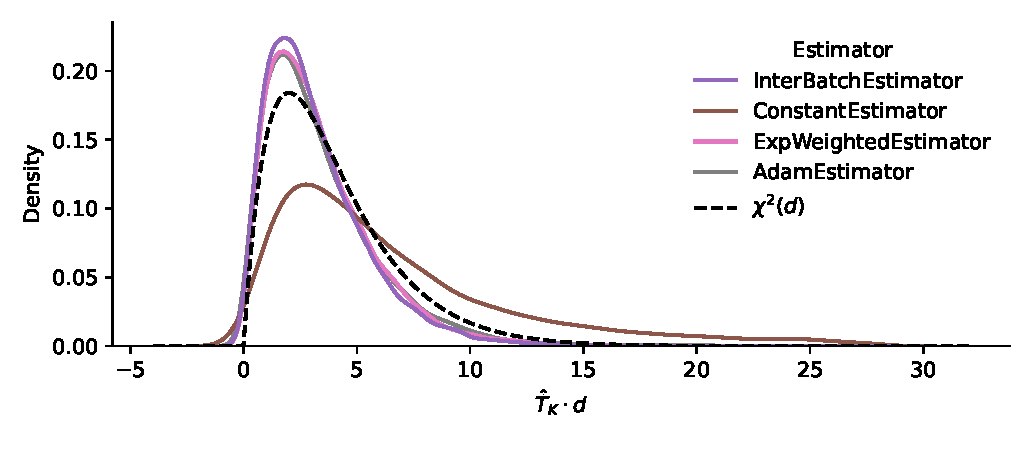
\includegraphics[width=\linewidth]{Figures/temperature_sum_chi2_comp.pdf}
    \caption{Observed distribution of $\hat{T}_k$ for the different variance estimation schemes, compared to the expected $\chi^2$ distribution.
The observed distributions extend below 0 only because of the KDE approximation used for plotting.}
    \label{fig:temperature_sum_chi2_comp}
\end{figure}
\begin{table}[htbp]
    \centering
    \begin{tabular}{lc}
\toprule
           Estimator & $\E[\hat{T}_K \in J_{T_K}(d, {0.99})]$ \\
\midrule
       AdamEstimator &                    $98.65 \pm 0.18~\%$ \\
   ConstantEstimator &                    $85.75 \pm 0.54~\%$ \\
ExpWeightedEstimator &                    $99.15 \pm 0.14~\%$ \\
 InterBatchEstimator &                    $99.01 \pm 0.15~\%$ \\
\bottomrule
\end{tabular}

    \caption{Values of $\hat{p}_{0.99}$ for the different gradient variance estimation schemes.}
    \label{tbl:temp_99}
\end{table}
The resulting distribution of $\hat{T}_K$ can be seen in \cref{fig:temperature_sum_chi2_comp}, compared to the expected $\chi^2$ distribution. 
We see that the distribution of $\hat{T}_K$ fits the expected distribution quite poorly for the sampler with $\beta=0$.
Introducing the various gradient estimators seems to result in the marginal distribution of $\hat{T}_K$ to match the correct distribution more closely.
However, there still seems to be some discrepancy compared to the expected $\chi^2$ distribution.
We see that the samplers with estimated variance are slightly underdispersing compared to the actual posterior. 
This underdispersion may indicate that we overestimate the variance and therefore do not inject sufficient noise compared to the momentum decay.
The $\hat p_{0.99}$ statistic is calculated in \cref{tbl:temp_99}, alongside a confidence interval based on the binomial distribution.
Looking at \cref{fig:est_variances_simulated} the estimation margin estimates also seem relatively uniformly distributed on the log scale, which would mean that we are generally overestimating more than we are underestimating in absolute terms.

\section{MNIST}
This section will explore the performance of the different methods on the MNIST dataset for classification. 
This dataset is often used to benchmark and compare different methods and implementations. 

In the SGHMC paper \cite{chen_stochastic_2014} they also compare against MNIST, using a small neural network with a single hidden layer of 100 units.
Using this model, they demonstrate comparable and even superior performance compared to SGD methods using weight regularization.
The authors of \cite{blundell_weight_2015} also compare with MNIST, only they use much larger networks with two hidden layers of sizes 400, 800, and 1200. 
They compare against regular SGD using dropout during training, showing slightly better test performance of VI.

This project compares these methods using a regular feed-forward neural network with two hidden layers of size 800, using ReLU as an activation function. 
We will be using a batch size of 128 for the optimization-based algorithms and 500 for the MCMC algorithms.
For the optimization based algorithm, we will be using the ADAM optimizer \cite{kingma_adam_2017}, with $\beta=(0.9, 0.999)$.
For the MCMC algorithms, we keep a sample for every epoch after a burn-in period of 50 epochs.
The different algorithms all have some hyperparameters that affect performance, some algorithms more than others.
To keep the comparison fair between the algorithms, the hyperparameter optimization framework Optuna \cite{akiba_optuna_2019} is used. 
This framework treats the choice of hyperparameters as a black-box optimization problem, trying to figure out what choices of parameters lead to the best validation error.

Another modeling choice is the question of parameter priors for the probabilistic methods. 
For the MCMC methods, we choose a hierarchal prior as in \cite{chen_stochastic_2014}. 
For each parameter group $\Theta_i=\{\theta_{i,1},\dots,\theta_{i,D_i}\}$, such as the bias or weight of some linear layer , we then use a Gaussian prior for the parameters $\theta_{i,j} \sim  \mathcal{N}(0, \sigma_i^2)$.
We then choose an uninformative prior for the variance parameters $1/\sigma_i^2 = \lambda_i \sim \Gamma(1,1)$.
This choice of prior enables different parameter groups to have parameter values on different scales.
In the MCMC framework, we can sample the precision parameters through a Gibbs step, using the conjugate distribution $p(\lambda_i | \Theta_i)$.
The sampling procedure then consists of sampling from parameter posterior conditioned on the precision using SGHMC and occasionally update the precision $p(\lambda_i | \Theta_i)$ using a Gibbs step.
As in \cite{chen_stochastic_2014}, we perform a Gibbs step after each epoch.

Since we are not able to a Gibbs step during the non-MCMC methods, we instead use a mixture of two Gaussian distributions,
\begin{align}
    \theta \sim t\cdot \mathcal{N}(0, \sigma_1^2) + (1-t)\cdot \mathcal{N}(0, \sigma_2^2),
\end{align}
as prior as proposed in the \cite{blundell_weight_2015}.
This allows for greater flexibility than a simple Gaussian, while not requiring us to optimize the prior of variance parameters as well.
We consider the parameters of the mixture prior as hyperparameters.
We, therefore, determine the particular values through hyperparameter search alongside the rest of the hyperparameters.

We run a hyperparameter search for 24 hours for each algorithm for the various hyperparameters. 
For each trial, the model train for 1000 epochs, and we use the resulting validation loss to measure the value of each choice of hyperparameters.  
Since the variational inference algorithm may be significantly slower than the other methods if using many samples for estimating the ELBO gradient, we impose a two-hour time limit for each training run. 
The hyperparameters are then set based on the top few results for each algorithm, and we train the model a final time.
The validation curves corresponding to the final training run for each algorithm can be seen in \cref{fig:mnist-best-val-curves}.
\begin{figure}[htbp]
    \centering
    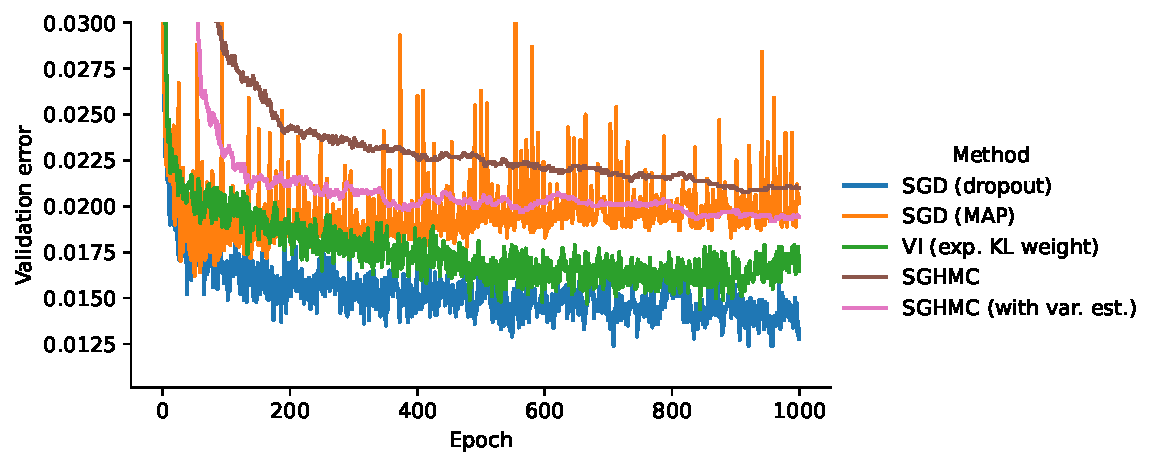
\includegraphics[width=\linewidth]{Figures/mnist-final-runs-val.pdf}
    \caption{Validation curves for final training runs of FFNN model on the MNIST dataset for each algorithm.}
    \label{fig:mnist-best-val-curves}
\end{figure}
Tables documenting the choice of parameters can be in \cref{apx:mnist-sweep}.
We choose to use the scheduled re-weighting of the KL-term for the VI algorithm, as we see it performing better than using the constant weight.

Some of the algorithms tended to overfit, so the best model during training according to validation error is chosen for the non-MCMC methods for calculating the test error.
The variational algorithm is allowed to train for longer, to see whether the performance increases if we let the model train for all 1000 epochs. 
The resulting testing errors for each algorithm can be seen in \cref{tab:mnist-test-err}.
\begin{table}[htbp]
    \centering
    \begin{tabular}{ll}
\toprule
{} & Test error incl. 95\% CI \\
\midrule
SGD (MAP)              &      $0.0175 \pm 0.0026$ \\
SGD (dropout)          &      $0.0143 \pm 0.0023$ \\
SGHMC                  &      $0.0173 \pm 0.0026$ \\
SGHMC (with var. est.) &      $0.0158 \pm 0.0024$ \\
VI (exp. KL weight)    &      $0.0155 \pm 0.0024$ \\
\bottomrule
\end{tabular}

    \caption{Test errors for the FFNN model on MNIST dataset.}
    \label{tab:mnist-test-err}
\end{table}
We see that out of the methods attempted, regular SGD with dropout wins out, however not by a lot. 
Interestingly, both SGHMC methods seem to perform significantly better than suggested by the validation error. 
Since we used the validation set for tuning our parameters, we would expect the opposite to be true. 
In any case, both the validation and test error seem to indicate that the SGHMC using gradient variance estimation improves the predictive performance of the models.

\subsection{Calibration}

As mentioned in the introduction, poorly calibrated deep learning models are not uncommon. 
A key motivator for experimenting with Bayesian methods has been to try and get a more robust and reliable estimator.
As in \cite{guo_calibration_2017} we use the \emph{expected calibration error} (ECE) for benchmarking the uncertainty of the different methods.
For some set of predictions, $\hat{y}$ the \emph{confidence} is defined as the estimated probability $\hat{p}$ of belonging to the estimated class.
The ECE statistic compares the confidence of the model to the observed accuracies.
According to the output confidence, we group the test observations into $M$ bins of size $1/M$. 
Then, the accuracy of each bin $B_m$, can be calculated as:
\begin{align}
    \acc(B_m) = \frac{1}{|B_m|}\sum_{i\in B_m}\bm{1}(\hat{y}_i = y_i)
\end{align}
Likewise, we calculate the average model confidence across the bin
\begin{align}
    \conf(B_m) = \frac{1}{|B_m|}\sum_{i\in B_m} \hat{p}_i.
\end{align}
Now, if the confidence of the model is to be trusted, we would expect $\acc(B_m) = \conf(B_m)$.
These measures thus gives us a way to benchmark the uncertainty of the model.
We then calculate the ECE as the expected absolute difference between the accuracy and the confidence weighted according to the size of each bin
\begin{align}
    \text{ECE} = \sum_{m=1}^{M} \frac{|B_m|}{n}|\acc(B_m)-\conf(B_m)|.
\end{align}
This gives us a single statistic to compare the inference methods across.
In \cref{tab:mnist-ece}, the ECE for the test set can be seen for each of the inference methods.
The accuracy and mean confidence of each bin can be seen in \cref{fig:mnist-calibration}. 
\begin{table}[htbp]
    \centering
    \begin{tabular}{lr}
\toprule
{} &   ECE \\
\midrule
SGD (dropout)          & 1.39\% \\
SGD (MAP)              & 1.00\% \\
VI (exp. KL weight)    & 0.77\% \\
SGHMC                  & 3.04\% \\
SGHMC (with var. est.) & 1.55\% \\
\bottomrule
\end{tabular}

    \caption{Estimated ECE on test set for the FFNN model trained on the MNIST dataset.}
    \label{tab:mnist-ece}
\end{table}
\begin{figure}[htbp]
    \centering
    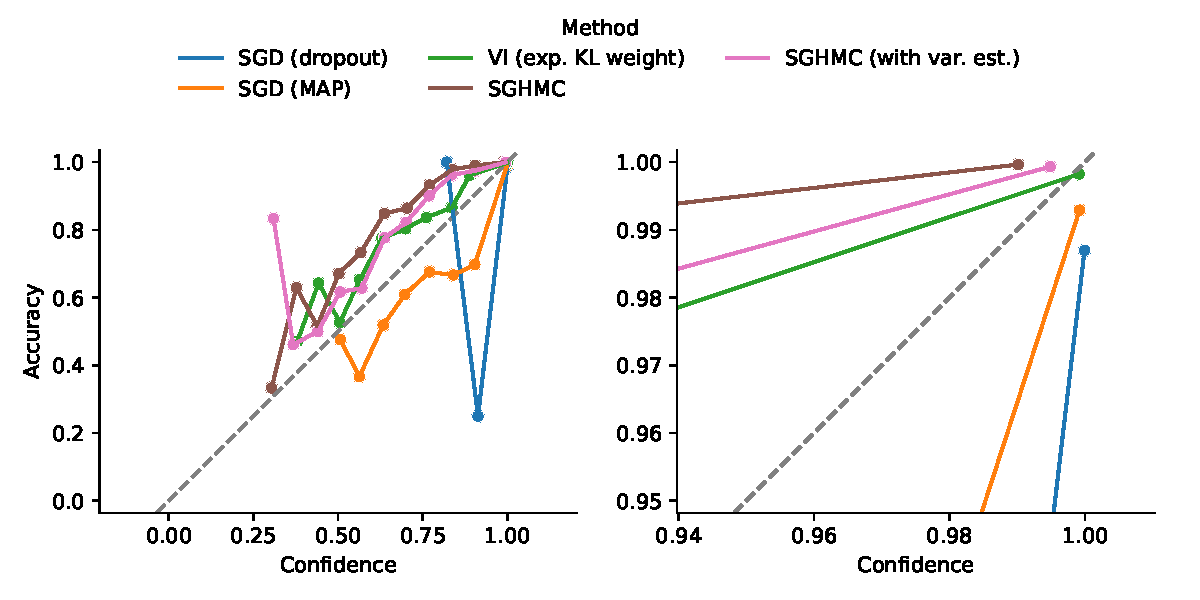
\includegraphics[width=\linewidth]{Figures/mnist-calibration.pdf}
    \caption{Accuracy and mean confidence across different bins for FFNN model trained on the MNIST dataset, for each algorithm.}
    \label{fig:mnist-calibration}
\end{figure}
According to the ECE, we see that VI leads to the most well-calibrated model, while the MCMC algorithms result in the most poorly calibrated models.

\subsection{Temperature Diagnostics}
As with the polynomial model, we can use the marginal distribution of the momentum variables $r$ to examine how well the sampled distribution resembles the correct distribution.
For each parameter group, we calculate the $\hat p_{0.99}$ statistic which can be seen in \cref{tab:mnist-temperatures}.
\begin{table}[htbp]
    \centering
    \begin{tabular}{ll}
\toprule
               Sampler &    $\hat{T}_{0.99}$ \\
\midrule
                 SGHMC & $66.67 \pm 0.84~\%$ \\
SGHMC (with var. est.) & $67.07 \pm 0.84~\%$ \\
\bottomrule
\end{tabular}

    \caption{Observed values of $\hat{p}_{0.99}$ during training of the FFNN model on the MNIST dataset.}
    \label{tab:mnist-temperatures}
\end{table}
We find that both of the sampling algorithms results in a value of this statistic of around $\hat{p}_{0.99}\approx 45\%$.
This value is a significant deviation from the expected $99\%$.
In \cref{fig:mnist-temperatures} we show the observed distribution of $\hat{T}_k$ compared to the expected distribution for each parameter group. 
We see that both samplers deviate from the expected $\chi^2$ distribution.
This indicates that the sampling procedure is breaking down to some extent and not correctly sampling from the posterior.
It is worth noting, that we optimized the choice of hyperparameters with respect to the validation error, which does not necessarily imply correctness of the samples from the posterior. 
\begin{figure}[htbp]
    \centering
    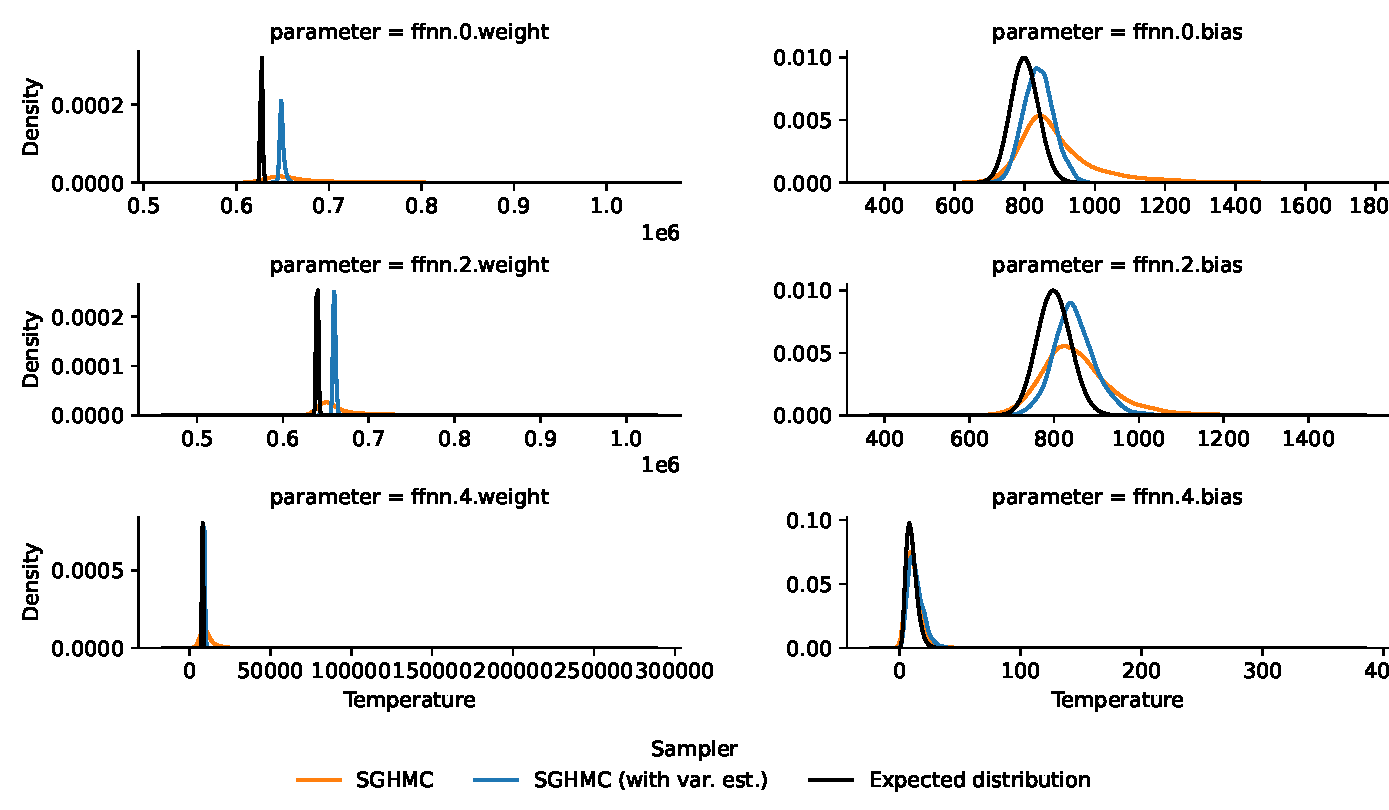
\includegraphics[width=\linewidth]{Figures/mnist-temperatures.pdf}
    \caption{Distributions of kinetic temperature, $\hat{T}_K$ for different parameter groups in the FFNN model during SGHMC training on the MNIST dataset.}
    \label{fig:mnist-temperatures}
\end{figure}

\FloatBarrier
\section{Convolutional Neural Network}

While we often use the combination of MNIST and feed-forward neural networks as a baseline, it is not the most representative example of advanced image analysis techniques.
In the following section, we investigate the performance of the different methods using a convolutional neural network (CNN) model and benchmarking against the more difficult CIFAR-10 dataset.

We initially fit a smaller CNN from scratch.
This model consists of three convolutional layers, each with 4o channels and a kernel size of 5.
Each convolution is followed by a batch normalization layer, a ReLU activation function, and a max-pooling layer.
These three composite layers are followed by a single linear layer of size 256, leading to the output.

The batch normalization layers are shown to improve training performance by reducing internal covariate shift and are commonly used for convolutional models \cite{ioffe_batch_2015}. 
However, due to the running moment estimates of the batch normalization layers, the probabilistic interpretation of the parameter estimates becomes less clear, and we therefore only include them for the models trained with dropout. 

We again use a burn-in period of 50 epochs for the sampling methods.
Instead of keeping a sample for every epoch, we now retain 200 samples.
We do this roughly uniformly, dynamically increasing the number of epochs between samples while pruning already retained samples.
We are using the same batch sizes as in the previous experiment.

We run hyperparameter search as with the previous experiment; however, we are now searching only for 12 hours combined with the use of an early-stopping criterion.
This criterion means that we finish the experiment and try another value during training if no improvement has been seen for the validation error for 15 epochs.
Based on the hyperparameters with the best performance, we choose the parameters seen in \cref{tab:cifar10-small-hparams} and train the models again. 
The hyperparameter search for the two SGHMC methods doesn't really show clear cut choices for either algorithm, and we therefore prioritize setting the same parameters across both methods for comparison. 
\begin{table}[htbp]
    \centering
    \begin{tabular}{p{4cm}p{9cm}}
        \toprule
        Algorithm & Parameters chosen \\ \midrule
        SGD (MAP) & 
        $\texttt{lr}=9 \times 10^{-4}$, 
        $\log\sigma_1=-2$, 
        $\log\sigma_2=-8$, 
        $\texttt{mixture\_ratio}=0.6$ \\ \midrule
        SGD (dropout) & $\texttt{lr}=9\times 10^{-4}$,
        $\texttt{dropout}=0.6$ \\ \midrule
        SGHMC & $\texttt{lr}=2\times 10^{-7}$, $\alpha=0.05$, $\texttt{resample\_momentum\_every}=10000$ \\ \midrule
        SGHMC (with variance estimate) &  $\texttt{lr}= 2 \times 10^{-7}$, 
        $\alpha=0.05$,
        $\texttt{estimation\_margin}=2$, $\texttt{resample\_momentum\_every}=10000$ \\  \midrule
        Variational inference &    
        $\texttt{lr}=5 \times 10^{-4}$,
        $\log\sigma_1=-1$,
        $\log\sigma_2=-8$,
        $\texttt{mixture\_ratio}=0.35$,
        $\texttt{n\_particles}=7$, constant KL weight \\
        \bottomrule
    \end{tabular}
    \caption{Chosen hyperparameters for the convolutional model on the CIFAR10 dataset.}
    \label{tab:cifar10-small-hparams}
\end{table}
For each method, the validation curves during the final training run can be seen in \cref{fig:cifar-small-final-runs-val}, and the resulting testing errors can be seen in \cref{tab:cifar10-small-test-err}.
\begin{figure}[htbp]
    \centering
    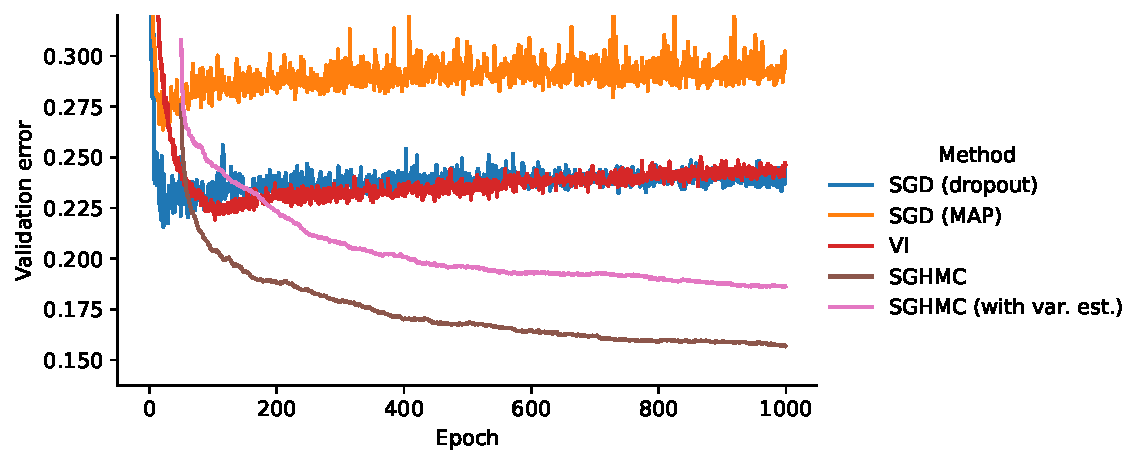
\includegraphics[width=\linewidth]{Figures/cifar-small-final-runs-val.pdf}    
    \caption{Validation curves for final training runs of convolutional model on the CIFAR10 dataset for each algorithm.}
    \label{fig:cifar-small-final-runs-val}
\end{figure}
{tab:cifar10-small-test-err}. 
\begin{table}[htbp]
    \centering
    \begin{tabular}{ll}
\toprule
{} & Test error incl. 95\% CI \\
\midrule
SGD (MAP)              &      $29.28 \pm 0.89~\%$ \\
SGD (dropout)          &      $24.88 \pm 0.85~\%$ \\
SGHMC                  &      $16.57 \pm 0.73~\%$ \\
SGHMC (with var. est.) &      $19.02 \pm 0.77~\%$ \\
VI                     &      $24.90 \pm 0.85~\%$ \\
\bottomrule
\end{tabular}

    \caption{Test errors for the convolutional model on CIFAR10 dataset}
    \label{tab:cifar10-small-test-err}
\end{table}
Here we see the MCMC methods outperform the other methods by some margin.
Of the two MCMC methods, the regular SGHMC without gradient variance estimation achieves better test error. 

The superior performance of the MCMC methods may partly be because of the early stopping criterion.
As we can see in the \cref{fig:cifar-small-final-runs-val}, the validation error is characterized by some variance.
This variance may lead to occasional significant one-time decreases to the validation error, resulting in the early stopping criteria stopping prematurely.
This may favor strategies with a rapid initial increase in performance and correspondingly disfavor slower strategies that may lead to better performance over time.

Another point relating to the fairness of comparing the methods is that the MCMC methods predict based on a far larger ensemble of different models.
In order to investigate the effect of the ensemble methods, we uniformly, without replacement, sample anywhere from 1 up to and including every sample from the MCMC ensemble, and measure the test performance as a function of the size of the ensemble. 
\begin{figure}[htbp]
    \centering
    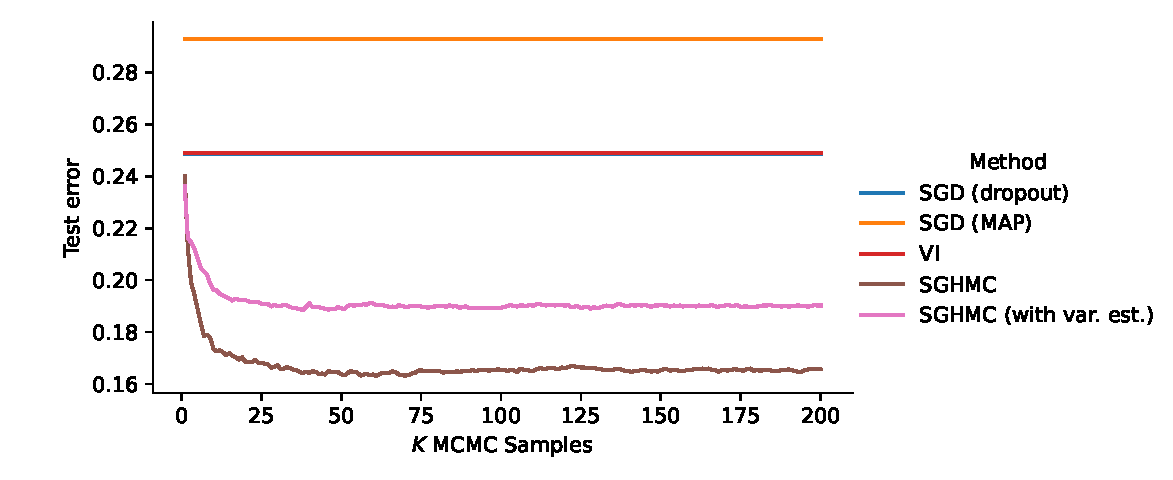
\includegraphics[width=\linewidth]{Figures/cifar-small-downsampling.pdf}
    \caption{Test performance for MCMC methods as a function of the size of the model ensemble.
    We show the test performance of the other methods as horizontal lines for comparison.
    Due to very similar test errors, the line corresponding to SGD with dropout is hiding underneath the line for VI.}
    \label{fig:cifar-small-downsampling}
\end{figure}
The corresponding error curves are shown in \cref{fig:cifar-small-downsampling}.
Here we see that the performance seems constant after $\approx 50$ samples, and even with only a single sample, both SGHMC algorithms outperform the other methods.

We also measure the ECE on the test set, to evaluate how well calibrated the models are.
The estimates can be seen in \cref{tab:cifar-small-ece}.
\begin{table}[htbp]
    \centering
    \begin{tabular}{lr}
\toprule
{} &    ECE \\
\midrule
SGD (dropout)          & 21.87\% \\
SGD (MAP)              & 18.47\% \\
VI                     &  3.62\% \\
SGHMC                  &  7.55\% \\
SGHMC (with var. est.) &  6.54\% \\
\bottomrule
\end{tabular}

    \caption{Estimated ECE on test set for the convolutional model trained on the CIFAR10 dataset.}
    \label{tab:cifar-small-ece}
\end{table}
Here we see that the probabilistic methods seem to be better calibrated than the SGD methods.
VI again results in the most well-calibrated model, now by some margin.
If we take a look at \cref{fig:cifar-small-calibration}, we also see that, while the SGD methods are generally way overconfident, the probabilistic methods tend to be underconfident.
\begin{figure}[htbp]
    \centering
    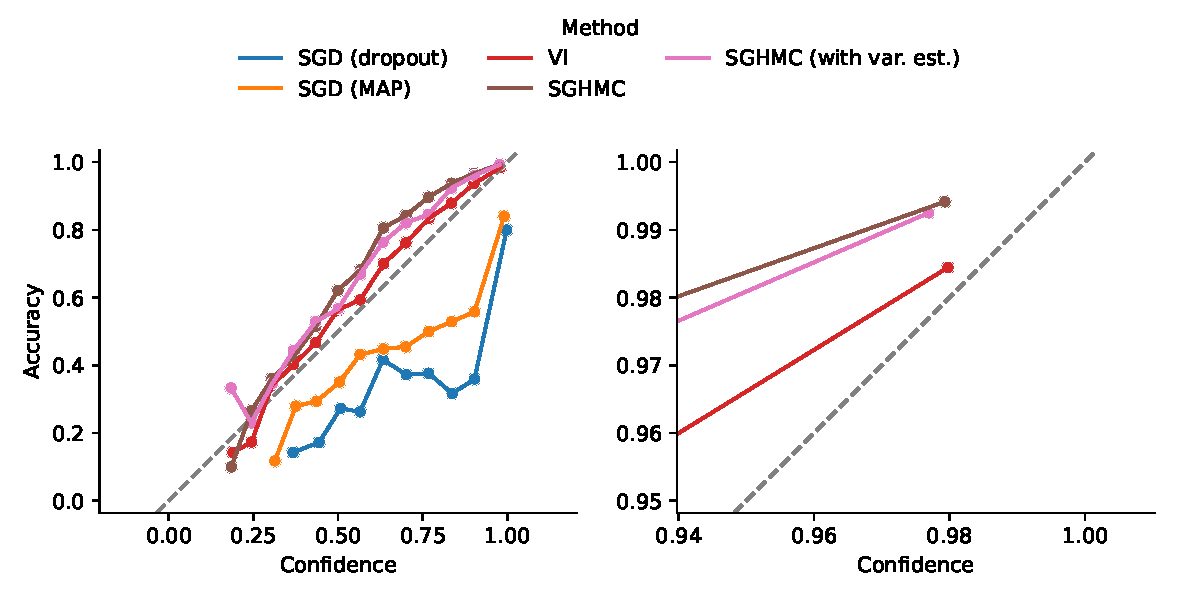
\includegraphics[width=\linewidth]{Figures/cifar-small-calibration.pdf}
    \caption{Accuracy and mean confidence across different bins for the convolutional model trained on the CIFAR10 dataset, for each algorithm.}
    \label{fig:cifar-small-calibration}
\end{figure}
Including the gradient variance estimator seems to result in a slightly lower estimated ECE for the SGHMC algorithm.

Again, we look at how well the distributional assumptions are met for the sampling algorithms.
In \cref{fig:cifar-small-temperatures} we see the observed distribution kinetic temperatures $\hat{T}_K$. 
In \cref{tab:cifar-small-temperatures}, we see the measured $\hat p_{0.99}$ values.
Also for this model, these values deviate some from the expected 99\%.
The $\hat p_{0.99}$ is a bit closer for the algorithm with variance estimation, however still not near 99\%.
\begin{table}[htbp]
    \centering
    \begin{tabular}{lc}
\toprule
                Method & $\E[\hat{T}_K \in J_{T_K}(d, {0.99})]$ \\
\midrule
                 SGHMC &                    37.24 $\pm$ 0.75~\% \\
SGHMC (with var. est.) &                    59.31 $\pm$ 0.76~\% \\
\bottomrule
\end{tabular}

    \caption{Observed values of $\hat{p}_{0.99}$ during training of the convolutional model on the CIFAR10 dataset.}
    \label{tab:cifar-small-temperatures}
\end{table}
\begin{figure}[htbp]
    \centering
    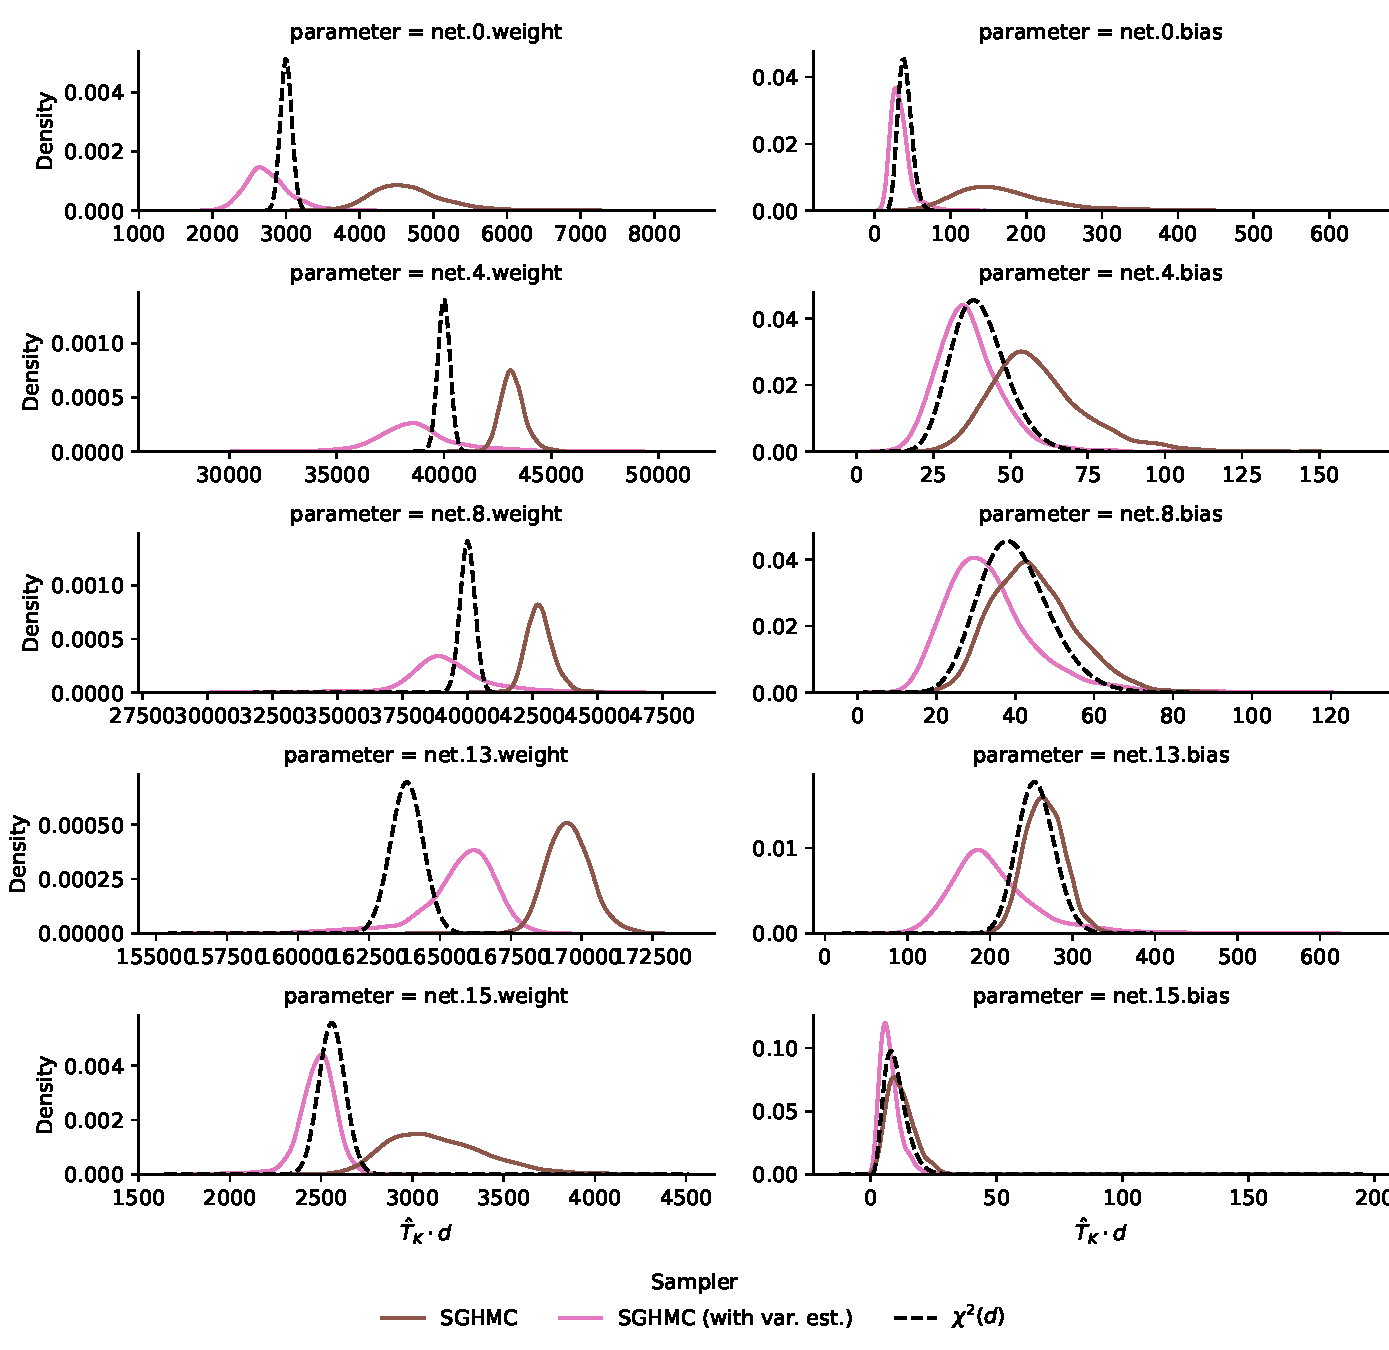
\includegraphics[width=\linewidth]{Figures/cifar-small-temperatures.pdf}
    \caption{Distributions of kinetic temperature, $\hat{T}_K$ for different parameter groups in the convultional model during SGHMC training on the CIFAR10 dataset.}
    \label{fig:cifar-small-temperatures}
\end{figure}

\FloatBarrier
\section{DenseNet}
Finally, we will be looking into how well the different methods handle even larger models.
As an example of a model of the larger variety, we look at training the DenseNet model \cite{huang_densely_2017}, specifically, the DenseNet-121 architecture. 
This model consists of 121 convolutional layers and is, as such, considerably larger than the previous convolutional model. 
We use a pre-trained model trained on ImageNet to start training using every method.

Due to the larger model and longer training time, we are not doing a hyperparameter search like the previous two models.
Instead, we try three different learning rates with every other hyperparameter fixed.
For the SGD and VI methods, we try learning rates of $2\times 10^{-4},5\times 10^{-4},1\times 10^{-3}$, and for SGHMC we try the learning rates $2\times 10^{-8},5\times 10^{-8},1 \times 10^{-7}$. 
We also try three different values for the dropout parameter for the SGD algorithm, 0, 0.3, and 0.6.

Each model gets to train for up to 1000 epochs, with a limit of 7 hours training time.
For this experiment, every algorithm uses a batch size of 128.
We choose the best value for the learning rate based on validation error.
The chosen learning are listed in \cref{apx:densenet-params} alongside the values set for the remaining hyperparameters. 
The validation error of each method during training can be seen in \cref{fig:cifar-densenet-val-err}, and the resulting test errors can be seen in \cref{tab:cifar-densenet-test-err}.
\begin{figure}[htbp]
    \centering
    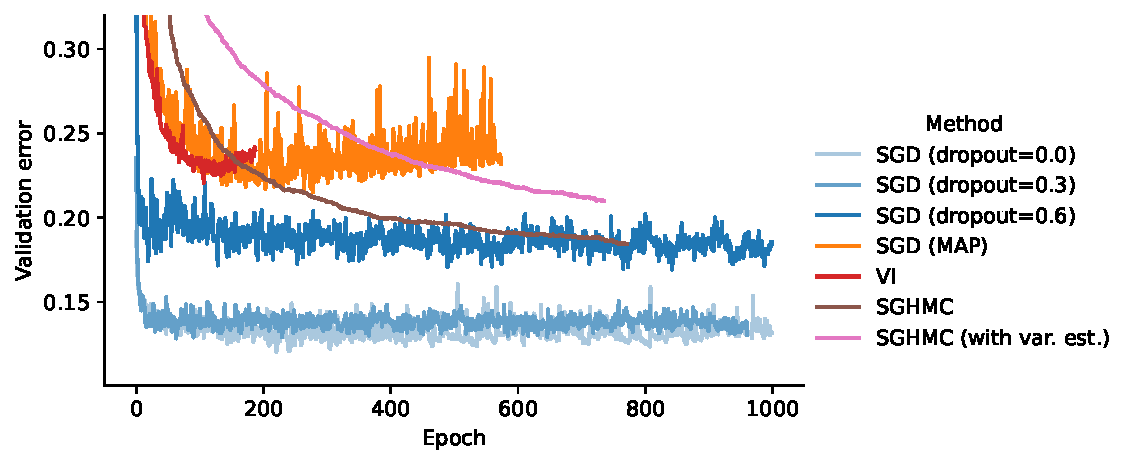
\includegraphics[width=\linewidth]{Figures/cifar-densenet-final-runs-val.pdf}
    \caption{Validation error during training for chosen parameters for DenseNet model on the CIFAR10 dataset.}
    \label{fig:cifar-densenet-val-err}
\end{figure}
\begin{table}[htbp]
    \centering
    \begin{tabular}{ll}
\toprule
                Method & Test error incl. 95\% CI \\
\midrule
             SGD (MAP) &      $23.36 \pm 0.83~\%$ \\
     SGD (dropout=0.0) &      $13.71 \pm 0.67~\%$ \\
     SGD (dropout=0.3) &      $14.01 \pm 0.68~\%$ \\
     SGD (dropout=0.6) &      $19.68 \pm 0.78~\%$ \\
                 SGHMC &      $18.96 \pm 0.77~\%$ \\
SGHMC (with var. est.) &      $21.17 \pm 0.80~\%$ \\
                    VI &      $24.32 \pm 0.84~\%$ \\
\bottomrule
\end{tabular}

    \caption{Test errors for the DenseNet model on CIFAR10 dataset}
    \label{tab:cifar-densenet-test-err}
\end{table}
We see that the models trained using regular SGD outperform the other methods, even when using a dropout rate of 0. 
This difference in performance may partly come down to the fact that we strip the model of its batch normalization layers to get a clear probabilistic interpretation of the parameter estimates.

Calibration statistics for the DenseNet model can be seen in \cref{tab:cifar-densense-ece} and \cref{fig:cifar-densenet-calibration}. 
\begin{table}[htbp]
    \centering
    \begin{tabular}{lr}
\toprule
{} &    ECE \\
\midrule
SGD (MAP)              & 15.62\% \\
SGD (dropout=0.0)      & 11.14\% \\
SGD (dropout=0.3)      & 11.75\% \\
SGD (dropout=0.6)      & 16.85\% \\
SGHMC                  & 10.33\% \\
SGHMC (with var. est.) &  9.46\% \\
VI                     &  8.77\% \\
\bottomrule
\end{tabular}

    \caption{Estimated ECE on test set for the DenseNet model trained on the CIFAR10 dataset.}
    \label{tab:cifar-densense-ece}
\end{table}
\begin{figure}[htbp]
    \centering
    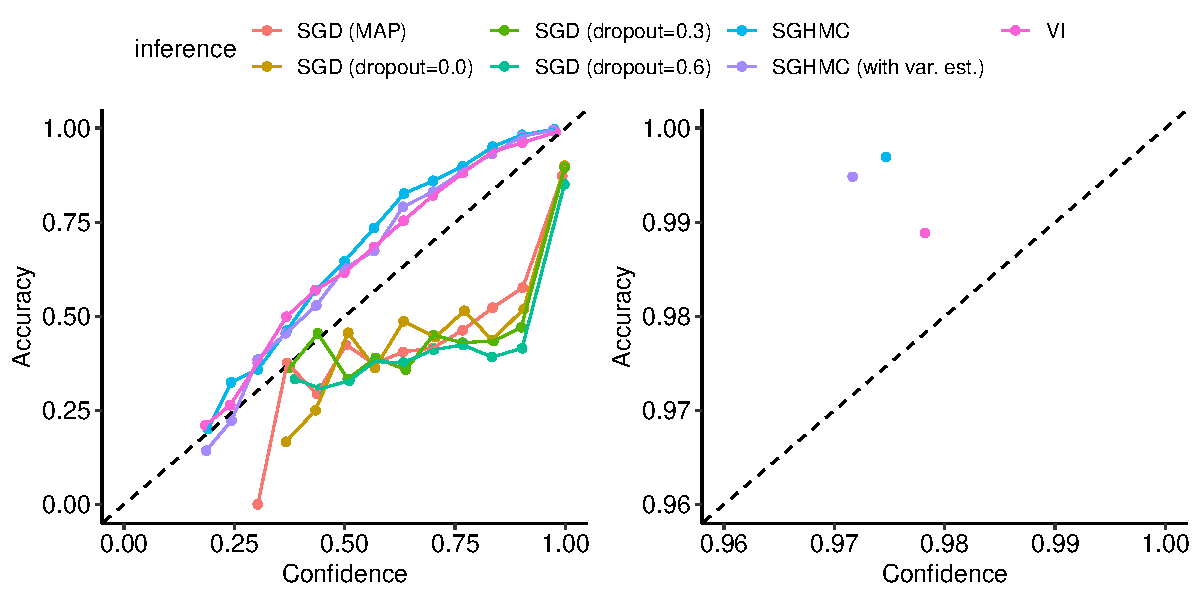
\includegraphics[width=\linewidth]{Figures/cifar10-densenet-calibration.pdf}
    \caption{Accuracy and mean confidence across different bins for DenseNet model trained on the CIFAR10 dataset, for each algorithm.}
    \label{fig:cifar-densenet-calibration}
\end{figure}
The probabilistic methods generally lead to better calibration than the SGD methods; however, neither results in particularly low ECE.  

As with the previous models, we use the $\hat p_{0.99}$ statistic as a diagnostic for the performance of our sampler.
This statistic is even worse than was the case for the other models.
As we see in \cref{tab:cifar-densenet-temperatures}, the $\hat p_{0.99}$ static is under 20\% for both sampling methods.
The distribution of $\hat{T}_K$ for 10 randomly sampled parameter groups can be seen in \cref{fig:cifar-densenet-temperatures}. 
We see that the observed distribution does not follow the expected $\chi^2$ distribution for any of the parameter groups shown. 
Curiously, for nine out of ten of the parameter groups, the distribution of the kinetic temperature is very similar across the two different samplers. 
The shape of the distribution is also very similar to the expected $\chi^2$ distribution, however shifted to hotter temperature.
\begin{table}[htbp]
    \centering
    \begin{tabular}{lc}
\toprule
                Method & $\E[\hat{T}_K \in J_{T_K}(d, {0.99})]$ \\
\midrule
                 SGHMC &                    12.41 $\pm$ 0.08~\% \\
SGHMC (with var. est.) &                    19.59 $\pm$ 0.10~\% \\
\bottomrule
\end{tabular}

    \caption{Fraction of observations of $\hat{T}_K$ falling in 0.99 confidence interval during training of  DenseNet model on CIFAR10.}
    \label{tab:cifar-densenet-temperatures}
\end{table}
\begin{figure}[htbp]
    \centering
    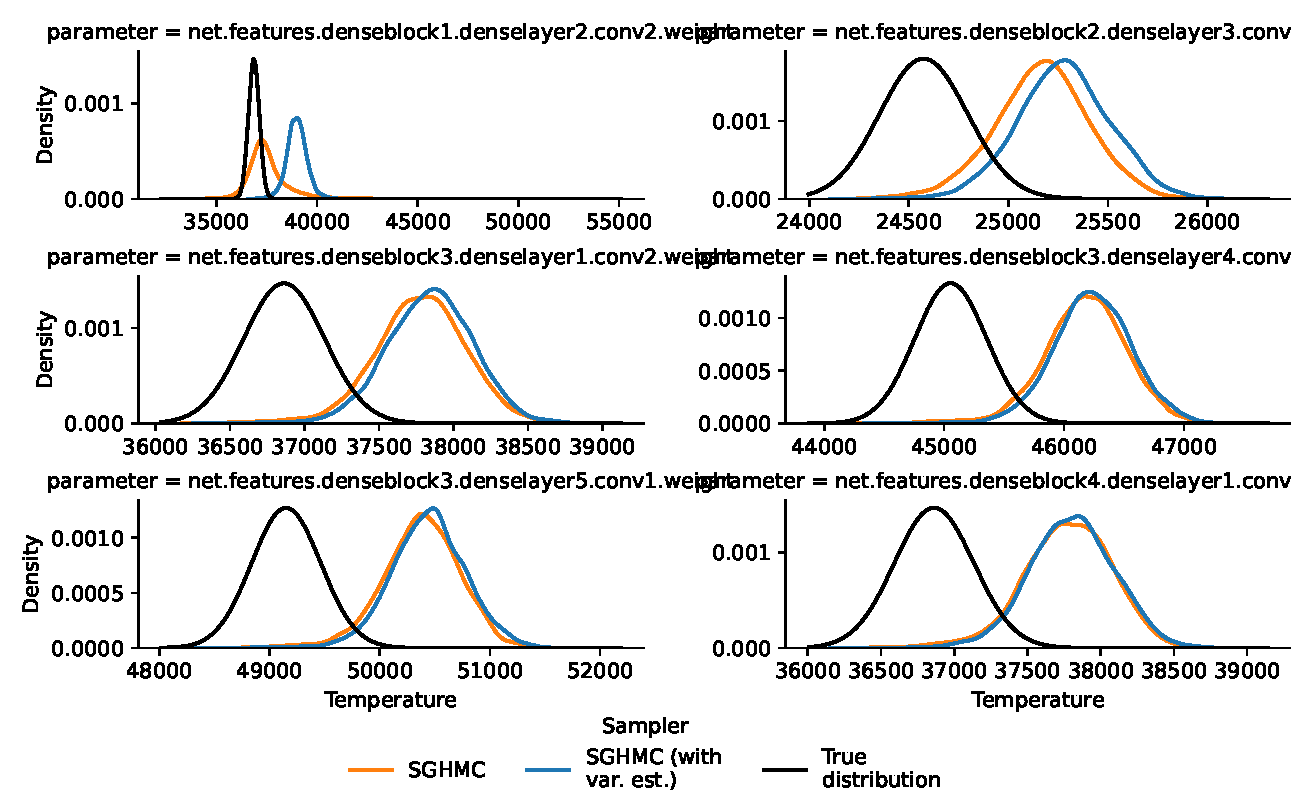
\includegraphics[width=\linewidth]{Figures/cifar-densenet-temperatures.pdf}
    \caption{Distribution of $\hat{T}_K$ during training for 10 randomly sampled parameter groups of DenseNet model on CIFAR10.}
    \label{fig:cifar-densenet-temperatures}
\end{figure}